
\documentclass[12pt,a4paper]{amsart}

% \usepackage{everypage}
% \usepackage[firstpage]{draftwatermark}
% \SetWatermarkScale{4}
% \SetWatermarkLightness{.95}

\usepackage{fullpage}
\usepackage{amsmath,amssymb}
%\usepackage{mathabx}
\usepackage{macros}
\usepackage{bm}
\usepackage{bbm}
\usepackage{mathtools}
\usepackage{bibentry}
\usepackage{hyperref}
\usepackage{graphicx}
\usepackage{tikz}

\usepackage{cleveref}

\newcommand{\OU}{\mathcal L}

% \newcommand{\exppi}[2]{\euler^{i\scalarof{#1}{#2}}}
% \newcommand{\expmi}[2]{\euler^{-i\scalarof{#1}{#2}}}
% \newcommand{\Basis}{(\Omega,\mathcal F,\Prob,(\mathcal F(t)_{t \ge 0}))}
% \newcommand{\frametop}[1]{\small\frametitle{\insertframenumber. #1}}
% \newcommand{\aval}[1]{\absoluteval{#1}}
% \newcommand{\cadlag}{C\`ADL\`AG}
% \DeclarePairedDelimiter{\ceil}{\lceil}{\rceil}
% \DeclarePairedDelimiter{\floor}{\lfloor}{\rfloor}

%% \renewcommand{\indicator}[1]{\mathbbmss 1 _{#1}}
%% \newcommand{\pspace}{(\Omega,\mathcal F,\Prob)}
%% \newcommand{\timeint}{\mathcal I}
%% \newcommand{\traj}{\mathcal T}

% \newcommand{\calF}{\mathcal F}
% \newcommand{\bu}{\bm u}
% \renewcommand{\S}{\mathbb S}
% \newcommand{\Sfunctions}{\mathcal S}
% \newcommand{\Dspace}[2]{\mathbb D^{#1,#2}}
% \newcommand{\bx}{\bm x}
% \newcommand{\by}{\bm y}
% \newcommand{\bz}{\bm z}
% \newcommand{\Mof}[1]{\operatorname{Mat}\left(#1\times#1\right)}
% \newcommand{\MRof}[2]{\operatorname{Mat}\left(#1\times#2\right)}
% \newcommand{\sym}[1]{\operatorname{Sym}(#1)}
% \newcommand{\psym}[1]{\operatorname{Sym}_+(#1)}
% \newcommand{\ppsym}[1]{\operatorname{Sym}_{++}(#1)}
% \newcommand{\GLof}[1]{\operatorname{GL}(#1)}
\newcommand{\one}{\bm 1}

\theoremstyle{plain}% default
\newtheorem{thm}{Theorem}%[section]
\newtheorem{proposition}[thm]{Proposition}
\newtheorem{npar}{}%[section]
\theoremstyle{definition}
\newtheorem{definition}{Definition}%[section]
\theoremstyle{remark}
\newtheorem{remark}{Remark}
\newtheorem{exercise}{Exercise}
\newtheorem{example}{Example}


\title{Probability 2021 \\ Part 1 \\
Probability on a finite sample space}
\author[G. Pistone]{Giovanni Pistone}
\address{de Castro Statistics, Collegio Carlo Alberto}
\email{giovanni.pistone@carloalberto.org}
\urladdr{https://www.giannidiorestino.it/}
\date{DRAFT \today}

\begin{document}
\maketitle

\begin{abstract}

\end{abstract}
These notes document lectures given in recent years at Collegio Carlo Alberto in Torino. The aim is to present the basics of Probability with emphasis on the special mathematical tools of interest in contemporary applications to Machine Learning and Artificial Intelligence. This live document and is frequently updated. Please check the date at the bottom of this page.

\tableofcontents

The set $\mathcal M=\mathcal M(\Omega,\mathcal A)$ of all probability measures on the measurable space $(\Omega,\mathcal A)$ is a convex set,
\begin{equation*}
    \mu,\nu \in \mathcal M \Rightarrow \forall \theta \in [0,1] \ (1-\theta) \mu + \theta \nu  \in \mathcal M \ .
\end{equation*}
Moreover, Jensen's inequality, 
\begin{equation*}
  \Phi\left(\expectat \mu f\right) \leq \expectat \mu {\Phi \circ f} \quad \text{if $\Phi$ is convex},  
\end{equation*}
is ubiquitous.

\begin{example}[Probability simplex] Each probability measure $\mu$ on
  $\Omega = \set{1,\dots,n}$ is uniquely characterized by its
  \emph{probability function} $p \colon j \mapsto p(j) =
  \mu(\set{j})$, $j=1,\dots,n$. The set of all probability functions
  is the \emph{probability simplex}, represented as a convex subset of
  $\reals^n$. Every probability function is the
  convex combination of the canonical basis.
\end{example}  

\begin{example}[Convex real functions] See
  \cite[p.~61--65]{rudin:1987-3rd}
Let $\phi$ be a real function defined on an open interval $I$. $\phi$ is
convex if for all $x,y \in I$ and all $\theta \in [0,1]$ it holds
\begin{equation*}
  \phi((1-\theta)x + \theta y) \leq (1-\theta)\phi(x) + \theta \phi(y) \ .
\end{equation*}

Other equivalent conditions obtain with $x=s$,
$u=y$, $t = (1-\theta)s + \theta u = s + \theta (u-s)$, $\theta \in
]0,1[$, that is $s
< t < u$: 
\begin{gather*}
  \frac{\phi(t)-\phi(s)}{t-s} \leq \frac{\phi(u)-\phi(s)}{u-s}  \\
    \frac{\phi(t)-\phi(s)}{t-s} \leq \frac{\phi(u)-\phi(t)}{u-t} 
\end{gather*}
The inequalities above imply that
\begin{equation*}
  t \mapsto \frac{\phi(t)-\phi(s)}{t-s}
\end{equation*}
is increasing and both left- and right-derivatives exists. In
particular $\phi$ is continuous. At each point $x$ there exist an $a$
between the left and the right derivative such that
\begin{equation*}
  \phi(y) - \phi(x) \geq a (y-x) \ .
\end{equation*}

If $\phi'$ exists, we have the equivalent conditions
\begin{equation*}
  \phi(y) - \phi(x) \geq \phi'(x)(y-x) \ , \quad \text{$\phi'$ is non-decreasing}
\end{equation*}

Relevant examples are
\begin{itemize}
\item  $I = \reals$, $x \mapsto \frac1a \avalof x ^ a$, $a \geq 1$;
  \item
  $I = \reals$, $x \mapsto \euler^x$;
\item $I = ]0,\infty[$, $x \mapsto - \log x$;
\item $I = ]0,\infty[$, $x \mapsto x \log x$.
\end{itemize}

As a first application, we consider the \emph{large deviation
  inequalities}. Let $f$ be a non-negative random variable on
$(\Omega,\mathcal A,\mu)$. As $x \geq c^{-1}(x \geq c)$ for all $x,c
\geq 0$, the monotonicity of the integral implies
\begin{equation*}
  c \mu(f \geq c) = \int c (f \geq c) \ d\mu \leq \int f \ d\mu \ .
\end{equation*}
Now, let $\phi \colon \reals_+ \to \reals_+$ be strictly
increasing. It follows
\begin{equation*}
  \mu(f \geq c) = \mu(\phi\circ f \geq \phi(c)) \leq \phi(c)^{-1}
  \int \phi\circ f \ d\mu \ . 
\end{equation*}
For example, take $\phi(x) = \euler^{ax}$, $a > 0$. It follows
\begin{equation*}
  \mu(f \geq c) \leq \euler^{-ac} \int \euler^{af} \ d\mu \ . 
\end{equation*}
Consider the model of the flipping of a fair coin $n$ times. The frequency of success $F_n$ has probability function $p(k/n) = \binom n k 2^{-n}$, $k=0,1,\dots,n$. The inequality becomes
\begin{equation*}
  \mu(F_n \geq 1/2 + \epsilon) \leq \euler^{-a(1+\epsilon)} \int \euler^{a F_n} \ d\mu =
  \euler^{-a(1/2+\epsilon)} \sum_{k=0}^n \euler^{ak/n} \binom n k 2^{-n} = 2^{-n}
  \euler^{-a(1/2+\epsilon)} \left(1 + \euler^{a/n}\right)^n \ .
\end{equation*}
Let us take the logarithm and minimize the RHS w.r.t. $a > 0$.
\begin{equation}\label{eq:LD-1}
  \log \mu(F_n \geq 1/2+\epsilon) \leq - \sup_{a > 0} \left(a(1/2 + \epsilon) - n \log\frac{1+\euler^{a/n}}2\right)
\end{equation}
We will finalize the computation later.

As a second application, we consider the \emph{entropy}. Let $\mu$ be a \emph{probability measure} on
$(X,\mathcal X)$. For each non-negative random variable $f \colon X$
define its entropy to be the excess in Jensen's inequality for a special convex function:
\begin{equation*}
  \entropyof{f} = \expectat \mu {\Phi\circ f} - \Phi\left(\expectat
    \mu f\right), \quad \text{where} \quad \Phi(y) = y \log y \ ,
\end{equation*}
if each term is well defined. Notice that the second term in the RHS is zero if $\expectat \mu f = 1$. In such a case, the mapping $\mathcal X \ni A \mapsto \expectat \mu {(A)f} = \int _A f \ d\mu$ is a probability measure.

The function $\Phi$ is continous
on $\reals_\geq$ as $\lim_{y \downarrow 0} y \log y = 0$ and has
derivatives given for $y > 0$ by
\begin{equation*}
  \Phi'(y) = 1 + \log y \ , \quad \Phi''(y)= 1/y \ .  
\end{equation*}
It is strictly convex with minimum value $-\euler^{-1}$ at
$\euler^{-1}$. The negative part of $\Phi\circ f$ is bounded by
$\euler^{-1}$, then $\expectat \mu {\Phi\circ f}$ is well defined,
possibly $+\infty$. Jensen's inequality gives
\begin{equation*}
  \Phi\left(\expectat \mu f\right) \leq \expectat \mu {\Phi\circ f} \ .
\end{equation*}
If the right-hand-side is finite, then the entropy is well
defined. Otherwise, one has to require $\expectat \mu f < \infty$. The
entropy is strictly positive, unless $f$ is constant.
\end{example}

\section{Probability functions}

\subsection{Convex sets}
\label{sec:aside:-convex-set}

Convex analysis is an important topic in applied probability. A
standard reference is the monograph \cite{barvinok:2002}.

A subset $H$ of a vector space $V$ is an \emph{affine space} if
$\setof{x-y}{x,y \in H}$ is a sub-vector space of $V$ which is called
the vector subspace parallel to $H$. The dimension of the affine space
$H$ is the dimension its parallel vector subspace. Given
$x_0,\dots,x_n \in V$ the set of all vectors of the form
$x_0 + \sum_{j=1}^n \lambda_j x_j$, $\lambda_j \in \reals$, is the
affine space generated by the given vectors. An affine space of
dimension $n-1$ in $\reals^n$ is an \emph{hyper-plane},

A subset $C$ of the vector space $V$ is \emph{convex} if for all
$x,y \in C$ all of the segment $(1-\lambda)x + \lambda y$,
$\lambda \in [0,1]$ belongs to $C$. The intersection of two convex
sets is convex. Given $x_0,\dots,x_n \in V$ the set of all
$\lambda_0 x_0 + \cdots +\lambda_n x_n$ with
$\lambda_0 + \cdots + \lambda_n = 1$ is the convex set generated by
the given vectors. Such a set is called a \emph{polytope} (or convex
polytope). Notice that
$\sum_{j=0}^n \lambda_j x_j = (1 - \sum_{j=1}^n \lambda_j) x_0 +
\sum_{j=1}^n \lambda_j x_j = x_0 + \sum_{j=1}^n \lambda_j(x_j-x_0)$
that is, the polytope is a part of the affine space generated. A
notable example of convex set is the \emph{half-space} of $v \in V$
such that $\scalarof c v \leq b$ with $c \in V$ and $b \in \reals$. A
finite intersection of half-spaces is a convex set called a
\emph{polyhedron}. See \cref{fig:polyhedron}.
\begin{figure}
  \centering
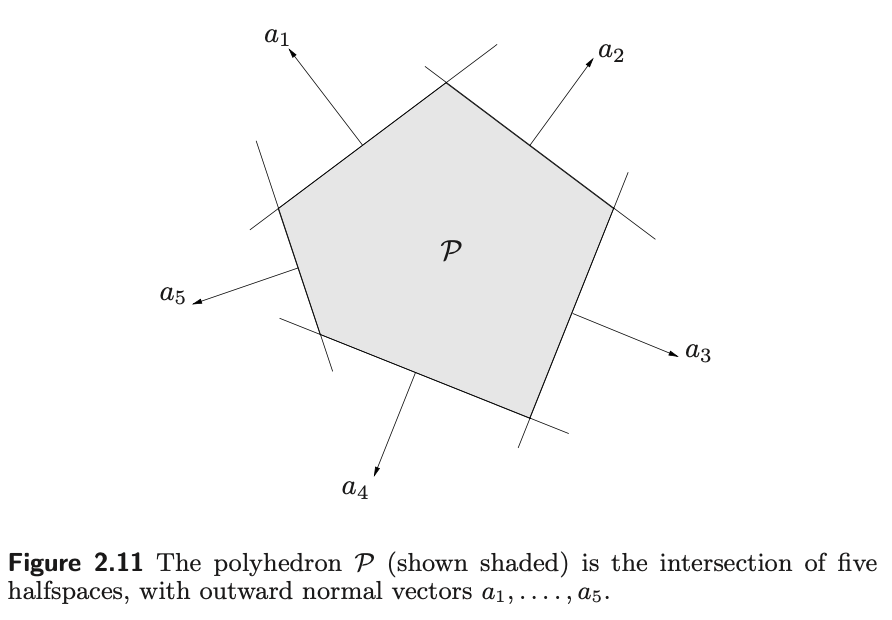
\includegraphics[width=.5\textwidth]{pictures/polyhedron.png}  
  \caption{Polyhedron from
    \href{https://math.stackexchange.com/questions/3522001/bounded-polyhedron-polytope}{mathexchange}
  }
  \label{fig:polyhedron}
\end{figure}
\emph{A bounded polyhedron is a polytope}. 

The vectors $x_0,\dots,x_m$ are \emph{affinely independent} if the vectors $x_1-x_0,\dots,x_m-x_0$ are linearly independent. They form a vector basis of the sub-space parallel to the generated polytope which in this case is called a \emph{simplex}. Two simplexes of the same dimension can be mapped one onto the other by an affine transformation that map their respective generators (the vertexes).    


\subsection{Affine geometry of the probability simplex}
\label{sec:probability-simplex}

Let $\lambda$ be a probability function on $\Omega$. As $\lambda \in \reals^\Omega$, we can write $\lambda = \sum_{x \in \Omega} \lambda(x) \delta_x$, so that the set $\Delta(\Omega)$ is the convex set generated by the probability functions associated to the Dirac probability measures. Let us code $\Omega$ as $\set{1,\dots,N}$ and write $\lambda= \sum_{j=1}^n \lambda_j e_j$. The vectors $e_j - e_m$, $j=1,\dots,N-1$ are linearly independent so that $\Delta(\Omega)$ is a special simplex which is called the \emph{probability simplex}. The parallel vector space is the vector space of the vectors of the form $\sum_{j=1}^n \alpha_j (e_j-e_1)$ that is of the form $\sum_{j=1}^n \alpha_j e_j$ with $\sum_{j=1}^n \alpha_j =0$. These are the vectors which are orthogonal to the constant vectors.

The set of probability functions with support $\Omega_1 \subset \Omega$ form a simplex of dimension $\# \Omega_1 -1$. If $\#\Omega_1 = n-1$ this sub-simplex is a \emph{face} of $\Delta(\Omega)$.

There is another simplex that represents the probability simplex $\Delta(\Omega)$ namely, the \emph{solid probability simplex}. In fact, we can represent a probability function by its $n-1$ values $\lambda_j,\dots,\lambda_{n-1}$ which form a vector in $\reals^{n-1}$ satisfying the conditions $\lambda_j \geq 0$ and $\sum_{j=1}^{n-1} \lambda_j \leq 1$. The vectors $e_1,\dots,e_{n-1},0 \in \reals^{n-1}$ are affinely independent and generate a simplex of dimension $n-1$ as $\sum_{J=1}^{n-1} \lambda_j e_j + \lambda_n 0$. The mapping between the two representations is given by $\reals^n \ni e_j \mapsto e_j \in \reals^{n-1}$ for $j=1,\dots,n-1$ and $\reals^n \ni e_n \mapsto 0 \in \reals^{n-1}$.

\begin{example}
  Study the probability simplex $\Delta(\set{1,2,3})$. In particular, construct the solid simplex and show it is a polyhedron. Consider the representation as an equilateral triangle. [Check for example the R p0lots in \url{https://www.r-bloggers.com/drawing-surface-plots-on-the-ir^3-simplex/}]
.\end{example}

\begin{example}[Probability simplex on $\Omega = \set{1,2}^2$] It is a simplex of dimension 3 with vertexes $\delta_i \otimes \delta_j$, $i,j = 1,2$. It is interesting to consider its graphical representations as a tetraedron. This example is especially instructive because of the product structure of the support. Check the Wikipedia entry \url{https://en.wikipedia.org/wiki/Simplex} for general cases. This allows the illustration of the effect of the push-forward.
\begin{figure}
  \begin{tabular}{ccc}
    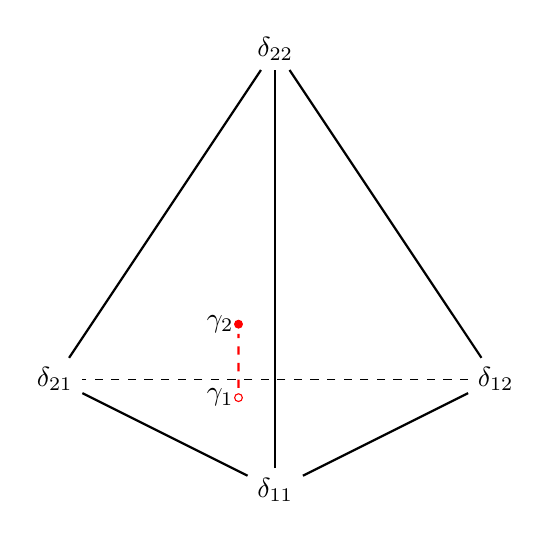
\begin{tikzpicture}[scale=2.8,baseline = (current bounding box.center)]
\node (n00) at (1,-.5) {$\delta_{11}$};
\node (n10) at (0,0) {$\delta_{21}$};
\node (n01) at (2,0) {$\delta_{12}$};
\node (n11) at (1,1.5) {$\delta_{22}$};
\node (K1) at (5/6,-1/12) {};
\node (gK1) at (5/6-1/12,-1/12) {$\gamma_1$};
\node (K2) at (5/6,1/4) {};
\node (gK2) at (5/6-1/12,1/4) {$\gamma_2$};
\draw[dashed] (n01) -- (n10);
\filldraw [red] (5/6,1/4) circle (.5pt);
\draw [red] (5/6,-1/12) circle (.5pt);
\foreach \from/\to in {n00/n10,n00/n01,n11/n10,n11/n01,n00/n11}
\draw[thick] (\from) -- (\to);
\draw [thick,red,dashed] (K1) -- (K2); % was: gray, dashed
\end{tikzpicture} & $\longrightarrow$ &
    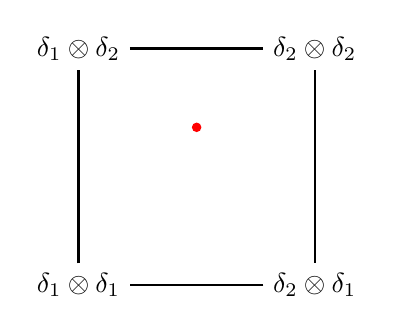
\begin{tikzpicture}[scale=3,baseline = (current bounding box.center)]
\node (n00) at (0,0) {$\delta_1\otimes\delta_1$};
\node (n10) at (1,0) {$\delta_2\otimes\delta_1$};
\node (n01) at (0,1) {$\delta_1\otimes\delta_2$};
\node (n11) at (1,1) {$\delta_2\otimes\delta_2$};
\foreach \from/\to in {n00/n01,n01/n11,n11/n10,n10/n00}
\draw[thick] (\from) -- (\to);
\filldraw [red] (1/2,2/3) circle (.5pt);
\end{tikzpicture}
  \end{tabular}
  \caption{The arrow is the marginalization function of the probability simplex $\Delta(\set{1,2}^2)$ to the product of the two marginal simplexes $\Delta(\set{1,2}) \times \Delta(\set{1,2})$. Each vertex of the left simplex is mapped to a vertex of the right polytope, $\delta_{ij} \mapsto \delta_i \otimes \delta_j$. The dashed segment from $\gamma_1$ to $\gamma_2$ represents the coupling polytope of the margins represented by the circle in the right polytope. Notice that $\gamma_1$ belongs to the facet opposite to $\delta_{22}$, while $\gamma_2$ belongs to the facet opposite to $\delta_{12}$.}\label{fig:2x2}
  \end{figure}
See \cref{fig:2x2} (taken from a papers). (Review the effect of the push forward on integrals and probability functions.) The dashed segment represents the set of \emph{couplings} $\mathcal P((1/2,1/2),(2/3,1/3))$. That is,
\begin{equation*}
  p_1(x) = (X_{\#} p)(x) = \sum_y p(x,y) \quad   p_2(y) = (Y_{\#} p)(y) = \sum_x p(x,y) 
\end{equation*}
and
\begin{equation*}
  \mathcal P(p_1,p_2) = \setof{q}{X_{\#} q = p_1,X_{\#} = p_2}
    \end{equation*}
    With the given margins,
    \begin{equation*}
      \begin{cases}
        q(1,1) + q(1,2) &= 1/2 \\
      q(2,1) + q(2,2) &= 1/2 \\
      q(1,1) + q(2,1) &= 2/3 \\
      q(1,2) + q(2,2) &= 1/3 
      \end{cases}
    \end{equation*}
From the 1st and the 3dr equation, take $q(1,1) = \theta$ as a parameter, the parametrized solution is
\begin{equation*}
  \theta \mapsto p_\theta =
  \begin{bmatrix}
    \theta & 1/2 - \theta \\ 2/3 - \theta & \theta - 1/6 
  \end{bmatrix} \ , 
  \quad \frac16 \leq \theta \leq \frac 12 \ .
\end{equation*}
The two end-points are
\begin{equation*}
\gamma_1 =
    \begin{pmatrix}
      1/6 & 1/3 \\ 1/2 & 0
    \end{pmatrix} \ , \quad \gamma_2 =
\begin{pmatrix}
  1/2 & 0 \\ 1/6 & 1/3
\end{pmatrix} \ .
\end{equation*}
for the \emph{cost} $c =
\begin{bmatrix}
  0 & 1 \\ 1 & 0
\end{bmatrix}$ the expected cost is
\begin{equation*}
 C(\theta) = \expectat \theta c = \sum_{x,y=1,2} c(x,y) p(x,y;\theta) = (1/2 - \theta) + (2/3 - \theta) = 5/6 - 2\theta
\end{equation*}
and the expected cost is minimum if $\theta = 1/2$. Such cost is
realized with the \emph{transport plan} $\gamma_2$.  The supports of
$\gamma_1$ and $\gamma_2$ have $2\cdot2-1 = 3$ arcs. The support of
$\gamma_2$ is a looped tree, while the support of $\gamma_1$ is not
because of the cycle $1 \rightleftarrows 2$.  The support of each
non-vertex coupling $\gamma = (1-\lambda)\gamma_1 + \lambda \gamma_2$,
$0 < \lambda < 1$, has $4$ arcs. For more information, check the keyword ``optimal transport.''
\end{example}

\subsection{Aside: differentials}
Let $f \colon \mathcal O \to \reals^n$, where $\mathcal O$ is an open sub-set of $\reals^m$. The function is differentiable at $\bar x \in \mathcal O$ if there exists a linear mapping $df(\bar x) \in L(\reals^m,\reals^n)$ such that
\begin{equation*}
f(\bar x + h) - f(\bar x) - df(\bar x)[h] = \smallo(h) \ .
\end{equation*}
The matrix representing the linear operator $df(\bar x)$ is called the Jacobian matrix of $f$, $Jf(\bar x)$, whose elements are the partial derivatives
\begin{equation*}
  Jf(\bar x) =
  \begin{bmatrix}
    \frac{\partial}{\partial x_j} f_i(x_1,\dots,x_n)
  \end{bmatrix}_{i=1,\dots,n; j=1,\dots m}
\end{equation*}

The derivative of the composite function $f \circ g$ at $x$ is $d(f\circ g)(x) = df(g(x)) \circ dg(x)$.

\subsection{Differentiability on the probability simplex} Let $I \ni \theta \mapsto \lambda(\theta)$ be a curve in the probability simplex  which is differentiable in $\reals^\Omega$. The derivative
\begin{equation*}
\lambda'(\theta) = \lim_{h \to 0} h^{-1} (\lambda(\theta+h) - \lambda(\theta)
\end{equation*}
belongs to the subspace parallel to the simplex. If $\lambda(\bar \omega;\bar \theta) = 0$, then the real differentiable function $\theta \mapsto \lambda(\bar\omega,\theta)$ has a minimum at $\theta=\bar\theta$, so that $\lambda'(\bar\omega,\bar\theta)=0$ and $\lambda'(\bar\theta)$ belong to the space parallel to the face of the simplex characterised by $\lambda(\bar\omega) = 0$.

\subsection{Aside: convex functions}

If a convex set $A \in \reals^m$ is open, then every straight line
intersects $A$ in an open interval or an empty interval. For example,
the subset of the solid probability simplex consisting of strictly
positive probability functions is an open convex set. The closure
$\overline A$ of an open convex set $A$ is a convex set. The
difference $\overline A \setminus A$ is the boundary of the convex
set.

\bigskip
\paragraph{Isolation theorem, Supporting hyperplane} \emph{Let $A$ be an open convex set in $\reals^m$ and let $x$ be in the border of $A$. There exists a unit vector $w$ such that  $\scalarof w {y-x} < 0$ for all $y \in A$ that is, the half-space contains the convex set}.

Let $x$ be a point of the boundary. A unit vector $u$ applied at $x$
enters $A$ if there is a $y \in A$ such that $u =
(y-x)/\normof{y-x}$. The set of all entering vectors cannot contain
two antipodal elements so that there is a unit vector $w$ such that
$\scalarof w u < 0$ for all entering unit vector. See a full proof in \cite[p
45-46]{barvinok:2002} and \cref{fig:hyperplanes}.\qed

\begin{figure}
  \centering
  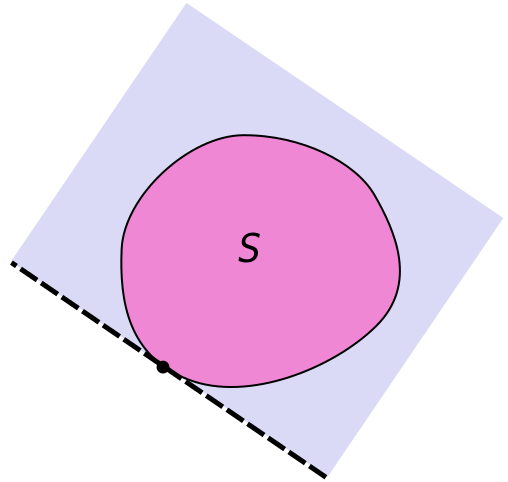
\includegraphics[width=.40\textwidth]{pictures/Supporting_hyperplane1.png} 
    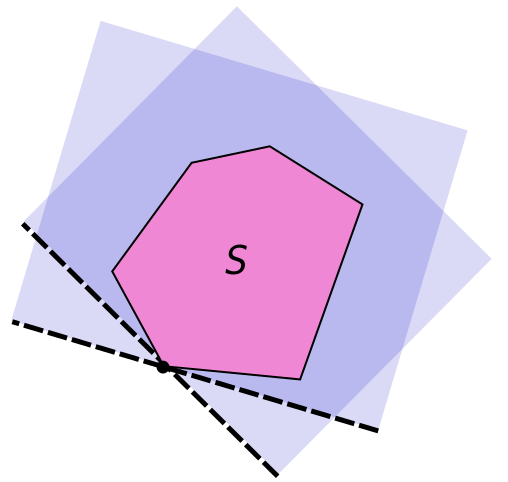
\includegraphics[width=.40\textwidth]{pictures/Supporting_hyperplane2.png}
  \caption{Supporting hyperplane from \href{https://en.wikipedia.org/wiki/Supporting_hyperplane}{Wikipedia}}
  \label{fig:hyperplanes}
\end{figure}

A function $\phi$ defined on on a domain in $\reals^n$ with values in
$\overline\reals = \reals \cup \set{+\infty}$ is convex if the
\emph{epigraph}
$\epiof \phi = \setof {(x,t)}{ x \in \domof \phi, t \in \reals,
  \phi(x) \leq t}$ is a convex subset of $\reals^{n+1}$. This
definition is equivalent to the standard one in case of finite values.

We define $\domof \phi$ to be the set where $\phi$ takes finite values. \emph{If $\phi$ is convex, then $\domof \phi$ is a convex subset of $\reals^n$.} If $x_1,x_2 \in \domof \phi$, then there exist $(x_1,t_1), (x_2,t_2) \in \epiof \phi$ and for all $\lambda \in [0,1]$ it holds $((1-\lambda)x_1+\lambda x_2,(1-\lambda)t_1+\lambda t_2) \in \epiof \phi$. In particular, $\phi((1-\lambda)x_1+\lambda x_2) < + \infty$. \emph{If $\phi$ is  convex, then $(1-\lambda)\phi(x_1) + \lambda \phi(x_2) \leq \phi((1-\lambda)x_1+\lambda x_2)$ for all $x_1,x_2 \in \reals^n$ and $\lambda \in [0,1]$.} If any of $x_1$, $x_2$ is not in $\domof \phi$ the inequality is trivially satisfied. Otherwise, it is the same computation as above. Conversely, if $\phi \colon \domof \phi \to \reals$ and $(1-\lambda)\phi(x_1) + \lambda \phi(x_2) \leq \phi((1-\lambda)x_1+\lambda x_2)$ for all $x_1,x_2 \in \domof \phi$ and $\lambda \in [0,1]$, then the function extended with value $+\infty$ outside the domain is convex.

Let $\phi$ be convex, and define the strict epigraph be open convex set
\begin{equation*}
\setof {(x,t)}{ x \in \domof \phi, t \in \reals, \phi(x) < t} \ .
\end{equation*}
Assume that at a point $(x,\phi(x))$ the entering unit vectors of the strict epigraph are not all horizontal. Then the Isolation Theorem implies that there exist at least a \emph{supporting hyper-plane}. In such a case, \emph{$\phi$ is the point-wise maximum of the supporting affine functions}. In the differentiable case, the tangent plane is the unique supporting hyperplane. If $\phi \in C^2(\mathcal O)$ then the Hessian matrix is non-negative definite.

\emph{Let $\phi$ be convex and let $\phi$ be differentiable on an open convex set $\mathcal O$. Then $\nabla \phi \colon \mathcal O \to \reals^n$ is \emph{monotone} i.e., $\scalarof {\nabla \phi(x) - \nabla \phi(y)}{x-y} \geq 0$ for $x,y \in \mathcal O$.} We can re-write the basic inequality as
\begin{equation*}
  \lambda^{-1}\left(\phi(x + \lambda(y-x))-\phi(x)\right) \leq \phi(y) - \phi(x) \ . 
\end{equation*}
If $\lambda \to 0$.
\begin{equation*}
  \scalarof{\nabla \phi(x)}{y-x} \leq \phi(y) - \phi(x) \ .
\end{equation*}
By adding the inequality with $x$ and $y$ exchanged we obtain the monotonicity.

Conversely, \emph{if $\phi$ is differentiable and $\nabla \phi$ is monotone on an open convex set $\mathcal O$, then $\phi$ is convex on $\mathcal O$.} Write $z = (1-\lambda)x + \lambda y$ and assume $0 < \lambda < 1$ because otherwise there is nothing to prove. observe that
\begin{multline*}
  \phi(z) - \phi(x) = \int_0^1 \scalarof {\nabla\phi(x + t (z-x))}{z-x} \ dt = \\
  \int_0^1 \scalarof {\nabla\phi(x + t (z-x)) - \nabla\phi(z)}{z-x} \ dt + \scalarof{\nabla\phi(z)}{z-x} \leq \\ \scalarof{\nabla\phi(z)}{z-x} = \lambda \scalarof{\nabla\phi(z)}{y-x} \ .
\end{multline*}
In fact, $z-x$ and $(x + t(x-z)) - z$ are proportional with factor $-(1-t) \leq 0$. In a similar way,
\begin{multline*}
  \phi(y) - \phi(z) = \int_0^1 \scalarof {\nabla\phi(z + t  (y-z))}{y-z} \ dt = \\
  \int_0^1 \scalarof {\nabla\phi(z + t (y-z))-\nabla\phi(z)}{y-z} \ dt + \scalarof{\nabla\phi(z)}{y-z} \geq \\ \scalarof{\nabla\phi(z)}{y-z} = (1-\lambda) \scalarof{\nabla\phi(z)}{y-x}\ ,
\end{multline*}
as $y-z$ and $(z+t(y-z)) - z$ are proportional with a factor $t \geq 0$. We rearrange the two inequalities as
\begin{align*}
  \phi((1-\lambda)x+\lambda y) &\leq \phi(x) + \lambda \scalarof{\nabla\phi(z)}{y-x} \\
  \phi((1-\lambda)x+\lambda y) &\leq \phi(y) + (1-\lambda) \scalarof{\nabla\phi(z)}{y-x} 
\end{align*}
and take the convex combination to conclude the proof.\footnote{This proof is taken from \cite[p. 26]{rockafellar:1970}}

\begin{example}[Examples of convex functions]
Show that the following functions are convex and compute the gradient mapping if it exists.
\begin{enumerate}
\item $\reals^n \ni x \mapsto \sum_{j=1}^n \aval{x_j}^a = \normat a x ^ a$, $a \geq 1$.
\item $\reals^n \ni x \mapsto \expof{\scalarof a x}$, $a \in \reals^n$.
\item $\reals^n \ni x \mapsto -\logof{\scalarof a x}$, $a \in \reals^n$.
\item $\reals_+ \ni x \mapsto x\log x$.
\end{enumerate}
\end{example}

\begin{example}[Convex conjugation] Let $\phi \colon \reals_+ \to \reals_+$ be strictly increasing and write $\psi=\phi^{-1}$. Write
\begin{equation*}
\Phi(x) = \int_0^x \phi(u) \ du  \qquad \Psi(y) = \int_0^y \psi(v) \ dv \ .
\end{equation*}
Extend with 0 when necessary. Then (make a picture!)
\begin{gather*}
    \Phi(x) + \Psi(y) \geq xy \quad \text{Fenchel's inequality}\\
    \Phi(x) + \Psi(y) = xy \quad \text{if $y = \phi(x)$ or $x = \psi(y)$} \quad \text{Legendre's equality}\\
    \Psi(y) = \sup_{x \geq 0} (xy - \Phi(x)) \quad \text{convex conjugation} 
\end{gather*}
Compare with \cref{eq:LD-1}. This can be generalised to $\reals^n$ using the last definition and the monotonicity of the gradient.
\end{example}

\subsection{Recap: density} Given a measure space
$(\Omega,\mathcal A, \mu)$ a non-negative measurable function $p$ is a
\emph{probability density} if $\int p \ d\mu = 1$. In such a case, the
mapping
\begin{equation*}
  p \cdot \mu \colon \mathcal A \ni A \mapsto \int_A p \ d\mu = \int (A) p\ d\mu
\end{equation*}
is a probability measure. Recall the notation for the indicator (aka
characteristic) function $(A) = \one_A = \chi_A$.

In fact. $p \cdot \mu (\emptyset) = 0$ because $(\emptyset) = 0$,
$p \cdot \mu(\Omega) = 1$ because $(\Omega) = 1$. If $(A_j)$ is a
sequence of disjoint events, then
$(\cup_j A_j) = \sum_j (A_j) = \sup_n \sum_{j=1}^n (A_j)$ and the
result follows from additivity and monotone continuy.

Given a mapping $X$ which is measurable from $(\Omega,\mathcal A)$ to
$(S,\mathcal S)$, the push-back of $\mathcal S$ is the
$\sigma$-algebra $X^{-1}(\mathcal S)$. \emph{A mapping
  $f \colon \Omega \to \reals$ is $X^{-1}(\mathcal S)$-measurable if,
  and only if, $f = \hat f \circ X$ for some $\hat f$ measurale on
  $(S,\mathcal S)$.} One direction is obvious. In the other direction,
one starts with the case $f = (A)$. The push-forward of $\mu$ is
$X_\sharp \mu = \mu \circ X^{-1}$. \emph{$\nu = X_\sharp \mu$ if, and
  only if, $\int_S \phi \ d\nu = \int_\Omega \phi \circ X \ d\mu$ for
  all non-negative measurable $\phi$.} Again, start the proof with the
case $\phi = (B)$.

The integral with respect to the push-forward of
a probability measure given by a density is computed as
follows. For $B \in \mathcal S$,
\begin{equation*}
  X_{\#} (p \cdot \mu) (B) = (p \cdot \mu)(X^{-1}(B)) = \int (X^{-1}(B)) p \ d\mu = \int (B)
\circ X p \ d\mu \ .
\end{equation*}
It follows, by linearity, that for each non-negative
simple function $\phi$ it holds
\begin{equation*}
  \int_\Omega \phi \circ X \ p \ d\mu = \int_S \phi \ dX_{\#} (p \cdot \mu) \ .
\end{equation*}
By approximation from
below the equality holds for all non-negative measurable function.
%  In
% conclusion, the push-forward measure is characterised by the
% \emph{change of variable} formula
% \begin{equation*}
%   \int f \circ X \ d\mu = \int f dX_{\#}\mu \ , \quad f \in \mathcal L^+
% \end{equation*}
% In the case the measure is actually a probability measure defined by a density $p$,
% \begin{equation*}
%  \int f \ d(X_{\#}p \cdot \mu) = \int f \circ X d (p \cdot \mu) = \int f \circ X p \ d\mu 
% \end{equation*}

\emph{Assume there exists a $\hat p$ such that the LHS equals
$\int \phi \circ X \ \hat p \circ X \ d\mu$.} Then, we can apply again the
change of variable for $\mu$, and get
\begin{equation*}
  \int \phi \ d(X_{\#} p \cdot \mu) = \int \phi \ \hat p \ dX_{\#}\mu = \int \phi d \ \hat p \cdot X_{\#} \mu \ .
\end{equation*}
As $\phi$ is arbitrary, we have computed the effect on the density of the push forward:
\begin{equation}\label{eq:push-forward-density}
  X_{\#}(p \cdot \mu) = \hat p \cdot X_{\#} \mu \quad \text{where} \forall \phi \in \mathcal L^+ \ \quad \int \phi \circ X p \ d\mu = \int \phi \circ X \hat p \circ X \ d\mu \ .
\end{equation}

Note that the arguments above are general, they do not depend on the
sample space being finite. The random variable $\hat p \circ X$ is the
\emph{conditional expectation} of $p$ to be discussed later. See
\cite[\S~IV.2]{malliavin:1995}, \cite[Ch.~23]{jacod|protter:2003}. It
is proved either by a projection argument, as in the quoted textbooks)
or by Radon-Nykodim theorem \cite[\S~6.10]{rudin:1987-3rd}.

A probability function $p$ is a density with respect to the counting measure. If $\Omega$ is finite, then the counting measure $\#(A) = \text{number of elements of $A$}$ is such that $\int_A p d\# = \sum_{\omega \in A} p(\omega)$. Consider now the push forward. \Cref{eq:push-forward-density} becomes
\begin{equation*}
  \int \phi \circ X \ p \ d\# = \sum_\omega \phi(X(\omega)) p(\omega) = \sum_{x \in \operatorname{Im}X} \phi(x) \sum_{x = X(\omega)} p(\omega) \ ,
\end{equation*}
which, in turn, gives $\hat p(x) = \sum_{x = X(\omega)} p(\omega)$. Usually, one writes $p_X$ to denote the push-forward density.

\begin{example}
  For $\Omega = \set{0,1}^n$ and $\theta \in ]0,1[$, define
  \begin{equation*}
    p(\omega) = p(x_1,\dots,x_n) = \prod_{j=1}^n \theta^{x_j} (1 - \theta)^{1-x_j} = (1-\theta)^n \left(\frac{\theta}{1-\theta}\right)^{\sum_j x_j} = \hat p \left(\sum_j x_j\right) \ ,
  \end{equation*}
with $\hat p(x) = (1-\theta)^n (\theta/(1-\theta))^x$. $p$ is a probability function because
\begin{equation*}
  \sum_{x_1,\dots,x_n = 0,1} \prod_{j=1}^n \theta^{x_j} (1 - \theta)^{1-x_j} = \prod_{j=1}^n (\theta + (1 - \theta))
  = 1 \ .
\end{equation*}
Consider now the mapping $X \colon \omega \ni (x_1,\dots,x_n) \mapsto \sum_j x_j \in S = \set{0,\dots,n}$. The push-forward of the counting measure is given by
\begin{equation*}
  \int \phi \circ X \ d\# = \sum_{x_1,\dots,x_n} \phi\left(\sum_j x_j\right)  = \sum_{x=0}^n \phi(x) \binom n x = \int \phi \ dX_\# \mu 
\end{equation*}
The push-forward of the \emph{Bernoulli} probability measure, that is, the probability measure with probability function $p$ is the \emph{Binomial} probability measure, that is, the probability measure with probability function $x \mapsto \binom n x \theta^x (1-\theta)^{n-x}$.
\end{example}

\subsection{Inequalities for the expectation}
\label{sec:ineg-expect}

If $u_1,\dots,u_n$ are real random variables, and $u$ denotes the corresponding random variable with values in $\reals^n$, then for each probability function $p$ the vector $\expectat p u = \sum_{\omega\in\Omega} p(\omega) u(\omega)$ is well defined. The operator $\Expectation_p$ is linear and affine, namely for vector random variables $u$, $v$, reals $\alpha$, $\beta$, and constant $b$, it holds
\begin{equation*}
  \expectat p {\alpha u + \beta v + c} = \alpha \expectat p u + \beta \expectat p v + b \ .
\end{equation*}

The basic convexity inequality is Jensen Inequality. \emph{Let $p$ be a probability function and let $u$ be a vector random variable. If $\phi$ is a convex function on $C$ and $C$ contains the image of $u$, then $\expectat p {\phi\circ u} \leq \phi\left(\expectat p u\right)$.} Here are two proofs, both interesting. First, observe that the convexity inequality can be easily generalised to any number of terms,
\begin{equation*}
  \phi\left(\sum_{j=1}^n \lambda_j x_i\right) \leq \sum_{j=1}^n \phi(x_j) \ , \quad \lambda_j \geq 0 \ , \sum_{j=1}^n \lambda_j = 1 \ ,
\end{equation*}
which is exactly the Jensen inequality written differently. Proof by recurrence. Second, let $x \mapsto a^tx + b$ be an affine function which is bounded by $\phi$. Then $a^t \expectat p u + b = \expectat p {a^tu+b} \leq \expectat p {\phi\circ u}$. Now take the supporting affine function at $\expectat p u$ that is, choose $a$ and $b$ such that $a^t \expectat p u + b = \phi\left(\expectat p u\right)$.

The most common example of application is with $\phi(x) = \sum_{j=1}^m \aval {x_j}^a = \normat a x ^a$, $a \geq 1$. It follows that
\begin{equation*}
  \expectat p {\sum_{j=1}^n \aval{u_j}^a} \geq \sum_{j=1}^n \expectat p {\aval{u_j}}^a \ .
\end{equation*}

Another inequality of interest is the H\"older Inequality: \emph{For all probability function $p$, all couple of random variables $X$ and $Y$, and all couple of positive numbers $a$ and $b$ such that $1/a+1/b = 1$, it holds}
\begin{equation*}
  \expectat p {XY} \leq \expectat p {\aval X ^a}^{1/a} \expectat p {\aval Y ^b}^{1/b}
\end{equation*}

\begin{example}[A proof of the H\"older inequality]
  Here is a proof involving computations of independent interest. From the convexity of $x \mapsto \euler^x$, that is
\begin{equation*}
  \left(\euler^u\right)^{1/a} \left(\euler^v\right)^{1/b} = \euler^{\frac1a u + \frac1b v} \leq \frac1a \euler^u + \frac1b \euler^v \ , 
\end{equation*}
we obtain
\begin{equation*}
  \expectat p {\left(\euler^u\right)^{1/a} \left(\euler^v\right)^{1/b}} \leq \frac1a \expectat p {\euler^u} + \frac1b \expectat p {\euler^v} \ .
\end{equation*}

Let $U$, $V$ be strictly positive random variables and define $u$ and $v$ by $\euler^u = U^a / \expectat p {U^a}$ and $\euler^v = V^b / \expectat p {V^b}$, respectively. Notice that now $\expectat p {\euler^u} = \expectat p {\euler^v} = 1$. The inequality above becomes
\begin{equation*}
  \expectat p {\left(U^a / \expectat p {U^a}\right)^{1/a} \left(V^b / \expectat p {V^b}\right)^{1/b}} \leq \frac1a \expectat p {\euler^u} + \frac1b \expectat p {\euler^v} = 1\ .
\end{equation*}
A little algebra produces the H\'older inequality for strictly positive random variable. Now consider $U + \epsilon$, $V+\epsilon$ and the limit $\epsilon\to0$ to prove the inequality for non-negative random variables. Finally, take $U = \aval X$ and $V = \aval Y$ and observe that $XY \leq \aval X \aval Y$ to conclude the proof.
\end{example}

\begin{example}[Convex conjugation]
If $\phi$ is increasing on $[0,\infty[$ and $\psi=\phi^{-1}$, then the two primitives $\Phi$ and $\Psi$ satisfy the Fentchel inequality
\begin{equation*}
    \Phi(x) + \Psi(y) \geq xy \ .
\end{equation*}
\end{example}

Another classical inequality is the Minkovski Inequality: \emph{For all probability function $p$, all couple of random variables $X$ and $Y$, and $a \geq 1$, it holds}
\begin{equation*}
  \expectat p {\aval{X+Y}^a} \leq \expectat p {\aval{X}^a} + \expectat p {\aval{Y}^a} \ . 
\end{equation*}

Minkovski inequality shows that \emph{$L(\Omega) \ni X \mapsto \expectat p {\aval X ^ a} ^{1/a} = \normat {p,a} X$ is a \emph{norm} if $p$ is strictly positive}. If $p$ is not strictly positive, then it is a \emph{semi-norm}.\footnote{It is interesting to compare this statement with the corresponding statement as seen in Measure Theory}

\begin{example}[Proof of Minkovski inequality]
The case $a=1$ has an immediate proof. If $a > 1$ use $(X+Y)^a = X(X+Y)^{a-1} + Y(X+Y)^{a-1}$ and H\"older inequality. Notice that $1/a+1/b=1$ if and only if $b = a/(a-1)$.  
\end{example}

\begin{example}[$L^2$-convergence and Weak LLN] Consider the Bernoulli $n$-scheme and define $S_n=X_1+\cdots+X_n$. Then $\expectat \theta {S_n/n} = \theta$ and $\expectat \theta {\left(\frac {S_n}n - \theta\right)^2} = \frac1n \theta(1-\theta) \to 0$ as $n \to \infty$.
\end{example}

\begin{exercise}[Cramer inequality] \label{ex:cramer}
Let $p$ be a probability function on $\Omega$, $X$ a non-constant real random variable, and $c \in \reals$. For all $t > 0$,
\begin{equation*}
  \probat p { X \geq c} = \probat p {tX \geq ct} = \probat p
  {\euler^{tX} \geq \euler^{ct}} \leq \frac1{\euler^{ct}} \expectat p {\euler^{tX}} = \expof{- \left(ct - \log\expectat p {\euler^{tX}}\right)} \ . 
\end{equation*}

The function $\kappa \colon t \mapsto \log \expectat p {\euler^{tX}}$ is convex with
\begin{equation*}
  \kappa'(t) = \frac{\expectat p {X \euler^{tX}}}{\expectat p {\euler^{tX}}} 
\end{equation*}
and
\begin{multline*}
  \kappa''(t) = \frac{\expectat p {X^2\euler^{tX}}\expectat p {\euler^{tX}} - \expectat p {X\euler^{tX}}^2}{\expectat p {\euler^{tX}}^2} = \\ \frac{\expectat p {\left(X - \expectat p {X \euler^{tX}}/\expectat p {\euler^{tX}} \right)^2 \euler^{tX}}}{\expectat p {\euler^{tX}}} > 0 \ .
\end{multline*}
To get a better understanding of the previous computation, let us define a family of probability functions
\begin{equation*}
  q(\omega;t) = \expectat p {\euler^{tX}}^{-1} \euler^{tX(\omega)} p(\omega) \ , \quad t >0 \ .
\end{equation*}
It is indeed non-negative and $\sum_\omega q(\omega;t) = \expectat p {\euler^{tX}} / \expectat p {\euler^{tX}} = 1$. Now
\begin{equation*}
  \kappa'(t) = \frac{\expectat p {X \euler^{tX}}}{\expectat p {\euler^{tX}}} = \expectat {q_t} {X} 
\end{equation*}
and
\begin{multline*}
  \kappa''(t) = \frac{\expectat p {X^2\euler^{tX}}\expectat p {\euler^{tX}} - \expectat p {X\euler^{tX}}^2}{\expectat p {\euler^{tX}}^2} = \\ \expectat {q_t} {X^2} - \expectat {q_t} X ^2 = \expectat {q_t} {(X - \expectat {q_t})^2} = \varat {q_t} {X} \end{multline*}

Note that $\kappa'(0) = \expectat p X$. We are interested in \emph{large deviation}, so that we assume $c > \expectat p X$.
To get the optimal inequality we look for the sup of a concave function,
\begin{equation*}
  \sup_{t > 0}{(ct - \kappa(t))} \ .
\end{equation*}
The derivative at 0 is
\begin{equation*}
  \left. \derivby t (ct - \kappa(t) \right|_{t=0} = c - \kappa'(0) = c - \expectat p X > 0 \ ,
\end{equation*}
hence
\begin{equation*}
  \sup_{t > 0}{(ct - \kappa(t))} \ .
\end{equation*}

Assume $\hat t$ is the solution of $c\hat t = \kappa'(\hat t)$, then
\begin{equation*}
  P_p(X \geq c) \leq \euler^{-(c\hat t - \log \expectat p {\euler^{\hat tX}})}
\end{equation*}

In particular, if $X$ is binomial, then
\begin{equation*}
  \expectat p {\euler^{tX}} = \sum_{k=0}^n \euler^{tk} \binom n k \theta^k (1-\theta)^{n-k} = (\theta \euler^t + (1 - \theta))^n 
\end{equation*}
so that
\begin{equation*}
  \kappa(t) = n \logof{\theta \euler^t + (1 - \theta)} \ , \quad \kappa'(t) = n \frac{\theta\euler^t}{\theta \euler^t + (1 - \theta)} \ .
\end{equation*}
The optimum value for the inequality is explicitly computable.

\emph{To be completed as second homework. Compute a bilateral bound, that is, a bound for $\probat p {\avalof{X - \expectat p X} \geq c}$ for $X$ binomial. Optionally, consider another example.}
\end{exercise}

\section{Exponential expression of the open simplex $\Delta^\circ(\Omega)$}
\label{sec:expon-expr-delt}

Every positive probability function is of the form $p(\omega) = \euler^{V(\omega)}$. This simple remark is frequently used in many applications as it provides a way to avoid inequality contrains. We start with some examples.

\begin{example}[The Bernoulli model as an exponential family]
  The Bernoulli model
  \begin{equation*}
 p(\omega;\theta) = \theta^{T(\omega)} (1-\theta)^{n-T(\omega)}
\end{equation*}
with $\theta \in ]0,1[$, $(X_1(\omega),\dots,X_n(\omega)) = \omega \in \Omega = \set{0,1}^n$, $X_j(\omega) = x_j$, $T(\omega) = \sum_{j=1}^n X_j(\omega)$, can be written as
    \begin{equation*}
      p(\omega;\theta) = \expof{\logof{\frac{\theta}{1-\theta}}T(\omega) + n\logof{1-\theta}} \ \quad \theta \in ]0,1[ \ .
    \end{equation*}
    For each $\omega$ the function $\theta \mapsto p(\omega;\theta)$ is called \emph{likelihood} of $\omega$.

    The parameter $\theta \in ]0,1[$ is the value of a probability or expected value, $\theta = P_p(X_j=1) = \expectat p {X_j}$. The new parameter $o = \theta/(1-\theta)$, $\theta = o/(1+o)$, represents the \emph{odds}, and $o \in ]0,+\infty[$.

    We use the parameter \emph{$\log$-odds}, $\alpha = \logof{\frac{\theta}{1-\theta}}$, $\theta = \euler^\alpha/(1+\euler^\alpha)$, $\alpha \in \reals$ so that we can write the Bernoulli model in the form
  \begin{equation*}
    p(\omega;\alpha) = \expof{\alpha T(\omega) - \kappa(\alpha)} \ , \quad \kappa(\alpha) = n \logof{1+\euler^\alpha} \ .
  \end{equation*}
The function $\kappa$ is strictly convex with
\begin{align*}
  \kappa'(\alpha) &= n\frac{\euler^\alpha}{1+\euler^\alpha} = n\theta = \expectat {p(\theta)} T \ ;\\
  \kappa''(\alpha) &= n\frac{\euler^\alpha}{(1+\euler^\alpha)^2} = n\theta(1-\theta) = \expectat {p(\theta)} {\left(T-n\theta)\right)^2} \ ; \\
  \kappa'''(\alpha) &= n \frac{\euler^\alpha(1-\euler^\alpha)}{(1+\euler^\alpha)^3} = \theta(1-\theta)^2 - \theta^2(1-\theta) \ .
\end{align*}

The \emph{$\log$-likelihood} at $\omega$ is
\begin{equation*}
 \ell \colon \alpha \mapsto \log p(\omega;\alpha) = \alpha T(\omega) - \kappa(\alpha) \ .
\end{equation*}
It is strictly concave with
\begin{equation*}
  \derivby \alpha \ell(\omega;\alpha) = T(\omega) - \kappa'(\alpha) = T(\omega) -  n \frac{\euler^\alpha}{1+\euler^\alpha} = T(\omega) - \expectat {p(\theta)} T \ ,
\end{equation*}
in particular, $\ell'(\omega;0+) = T(\omega)$ and $\ell(+\infty) = -\infty$. The maximum obtains at $\hat\theta(\omega)$ such that $T(\omega) = \hat\theta(\omega)$ that is, $\hat \theta(\omega) = T(\omega)/n$.

The random variable $\hat \theta$ is the \emph{maximum likelihood estimator} of the parameter $\theta$. This estimator is \emph{unbiased} because $\expectat {p(\theta)} {\hat \theta} = \theta$ and it is \emph{weakly consistent} because
\begin{equation*}
\probat {p(\theta)} {\aval{\hat \theta - \theta} \geq \epsilon} \leq \epsilon^{-2} \expectat {p(\theta)} {\left(\hat \theta - \theta\right)^2} = \epsilon^{-2} \frac{\theta(1-\theta)}{n^2} \to 0 \quad \text{if} \quad n\to\infty .
\end{equation*}
The behaviour of the standardized error i.e., the CLT will be discussed later.
\end{example}

The exercise above provides the simplest example of classical Statistics and the simplest example of the expression of a parametrized probability function as an \emph{exponential family}. The next exercise shows the use of weight functions. 
\begin{example}
Consider the binomial probability function
\begin{equation*}
  p(k;\theta) = \binom n k \theta^k (1-\theta)^{m-k} \ , \quad k \in \set {0,1,\dots,n} \ , \quad \theta \in ]0,1[ \ .
\end{equation*}
Here, the binomial factor does not depend on the parameter. It is convenient to consider the function $k \mapsto \binom n k$ as a \emph{weight function} on the sample space and write the exponential expression as
\begin{equation*}
  p(\theta) = \expof{\logof{\frac{\theta}{1-\theta}} K + n \logof{1-\theta}} \binom n K \ .
\end{equation*}
Now, the interesting factor is the \emph{density} with respect to the binomial weight, $\euler^{\alpha K - \kappa(\alpha)}$, $\alpha$ being the $\log$-odds.
\end{example}

A similar model has been considered in Statistical Physics a long time before its use in Statistics. In the next example, we use an \emph{un-normalised probability function} e.i., a function $f \colon \Omega \to \reals_+$. Given such a function, one computes the \emph{normalizing constant} $Z = \sum_{\omega\in\Omega} f(\omega)$ and $p = f/Z$ is a probability function. The set of all un-normalized probability function is a \emph{pointed cone} and the normalization is a mapping from the cone to the probability simplex.

\begin{example}[Gibbs distribution]
  If $\Omega$ is a finite set of states of a physical system, and $\omega \mapsto U(\omega)$ is a non-negative function whose value is the energy of the state $\omega$, the probability function
  \begin{equation*}
    p(\omega;t) \propto f(\omega) = \expof{-\frac{U(\omega)}t} \ , \ t > 0 \ ,
  \end{equation*}
  provides a probability on the set of states $\Omega$ which is called \emph{Gibbs distribution}. C.f. \cite[\S 28]{landau|lifshits:1980}. The parameter $t$ represents the absolute temperature.

The normalising constant is
\begin{equation*}
 Z(t) = \sum_{\omega\in\Omega} \expof{-\frac{U(\omega)}t} \ , 
\end{equation*}
so that the Gibbs probability function is
\begin{equation*}
  p(\omega;t) = \frac{\expof{-\frac{U(\omega)}t}}{\sum_{\omega\in\Omega} \expof{-\frac{U(\omega)}t}} = \expof{-\frac{U(\omega)}t - \log Z(t)} \ .
\end{equation*}
One has
\begin{equation*}
  \derivby t \log Z(t) = \frac {\sum_{\omega\in\Omega} \expof{-\frac{U(\omega)}{t}}\frac{U(\omega)}{t^2}}{Z(t)} = \frac1{t^2} \sum_{\omega\in\Omega} U(\omega) p(\omega;t) = \frac1{t^2} \expectat {p(t)} {U} \ 
\end{equation*}
and
\begin{equation*}
  \derivby t \log p(\omega;t) = \frac1{t^2} U(\omega) - \frac1{t^2} \expectat {p(t)} {U} \ .
\end{equation*}

Other equations similar to those we have obtained for the Bernoulli distribution hold. This provides the basic formalism for this physical model. For example, the deviation of the energy from its mean value is
\begin{equation*}
  U - \expectat {p(t)} {U} = t^2 \derivby t \log p(t) \ .
\end{equation*}
\end{example}

\subsection{Positive probability functions} In general, if the probability function $p : \Omega$ is positive, it is always possible to write it as $p(u) = \expof{U(\omega) - \kappa(U)}$, where $U$ is a random variable and $\psi(U)$ is constant depending on $U$. In fact, if $\log p(\omega) = U(\omega) - \kappa(U)$, then $U$ is identified up to a constant and, for any given $U$,
  \begin{equation*}
    1 = \sum_{\omega \in \Omega} p(\omega) = \euler^{-\kappa(U)} \sum_{\omega\in\Omega} \euler^{U(\omega)} \quad \text{so that,} \quad \kappa(U) = \logof{\sum_{\omega\in\Omega} \euler^{U(\omega)}} \ .
  \end{equation*}

  \begin{example}
  Condider the binomial probability function $p(k) = \binom n k \theta^k (1-\theta)^{n-k}$, $k = 0,\dots, n$, $\theta \in ]0,1[$, we can write
  \begin{equation*}
    p(k) = \binom n k (1-\theta)^n \left(\frac \theta {1-\theta}\right)^k = \expof{\log \binom n k + k \logof{\frac \theta {1-\theta}} + n \logof{1-\theta}}
  \end{equation*}
  that is, $U(k) = \log \binom n k + k \logof{\frac \theta {1-\theta}}$ and $\kappa(U) = - n \logof{1-\theta}$. 

  It is convenient to change the parameter: if $\alpha = \logof{\frac \theta {1-\theta}}$, then $\theta = \frac{\euler^\alpha}{1+\euler^\alpha}$ and
  \begin{equation*}
  p(k) = \expof{\alpha k + \log\binom n k - n \logof{1+\euler^\alpha}} \ .  
\end{equation*}
In fact, $U(k) = \alpha k + \log \binom n k$, hence
\begin{equation*}
  \kappa(U) = \logof{\sum_{k=0}^n \euler^{U(k)}} = \logof{\sum_{k=0}^n \binom n k \alpha^k} = n \logof{1+\euler^\alpha} \ .
\end{equation*}
\end{example}

Such a way to express probability functions and the related formalism was initiated in Statistical Physics by J.W. Gibbs (1901).

The mapping $U \mapsto p = \euler^{U - \kappa(U)}$ cannot be injective because the vector space of random variables has dimension $\#\Omega$ while the convex set of probability functions has dimension $\#\Omega - 1$. Precisely,
\begin{equation*}
  \euler^{U(\omega)-\kappa(U)} = \euler^{V(\omega) - \kappa(V)} \quad \Rightarrow U(\omega)-V(\omega) = \kappa(V) - \kappa(U) \ .
\end{equation*}

The function $\euler^U$ is a generic positive function and the set of positive functions is a cone. A base of this cone is the open probability simplex and the normalization is a projection onto this basis.

There are many ways to add a one-dimensional constraint to obtain a 1-to-1 function. 

\subsection{Potentials in the space parallel to the simplex}

\emph{For each positive probability function there is a unique potential $U$ such that $\sum_{\omega \in \Omega} U(\omega) = 0$.} Assume $p = \expof{U - \kappa(U)}$ with $\sum_{\omega \in \Omega} U(\omega) = 0$. Then
\begin{equation*}
  \sum_{\omega\in\Omega} \log p(\omega) = \sum_{\omega \in \Omega} U(\omega) - \kappa(\omega) = N \kappa(U) \ , \quad N = \# \Omega \ ,
\end{equation*}
that is, $\kappa(U) = \frac1N \sum_{\omega\in\Omega} \log p(\omega)$. Conversely, given any positive probability function, we can define $U = \log p - \frac1N \sum_{\omega\in\Omega} \log p(\omega)$ so that, $\sum_{\omega} U(\omega) = 0$. Moreover,
\begin{equation*}
  p = \expof{\log p} = \expof{U + \frac1N \sum_{\omega\in\Omega} \log p(\omega)} = \expof{U - \kappa(U)} 
\end{equation*}
with $k(U) = - \frac1N \sum_{\omega\in\Omega} \log p(\omega)$. In conclusion: \emph{Let $B_0$ denote the vector space parallel to the simplex. The mapping $B_0 \ni U \mapsto \euler^{U-k(U)}$ with $\kappa(U) = - \frac1N \sum_{\omega\in\Omega} \euler^{U(\omega)}$ is 1-to-1. The inverse of this mapping is}
  \begin{equation*}
    \Delta^\circ(\omega) \ni p\mapsto \log p - \frac1N \log p(\omega) \ .
  \end{equation*}

A similar, but more general and more useful computation, considers the case of an exponential density with respect to a weight function.

  \subsection{Potential centered at the probability function}
\label{sec:potent-cent-at}

Consider now the mapping
\begin{equation*}
  \Delta^\circ(\Omega) \ni p \mapsto V = \log p - \expectat p {\log p} \ .
\end{equation*}

Notice that
\begin{equation*}
  - \expectat p {\log p} = - \sum_{\omega\in\Omega} p(\omega) \log p(\omega) = H(p)
\end{equation*}
is the entropy of $p$, that is in this case $p = \euler^{V + H(p)}$.

\subsection{Non-negative potential}
\label{sec:non-negat-potent}

Consider the set $\mathcal U$ of all non-negative real functions $U : \Omega$ such that $\min U = 0$. Notice the peculiar shape of such a sub-set on $\reals^\Omega$: it is a pointed non-convex cone that is, if $U \in \mathcal U$ then $\rho U \in \mathcal Y$ for all $\rho \geq 0$ and moreover it is contained in the half-space associate to $B_0$.

The expression is unique, because of all the $U$'s such that $p = \euler^{U-\kappa(U)}$ only one belongs to $\mathcal U$.
  
In this expression, if $\Omega_0 = \setof{\omega \in \Omega}{U(\omega)=0}$ and $\Omega_+ = \setof{\omega \in \Omega}{U(\omega) > 0}$, then
  \begin{equation*}
 \kappa(U) = \log \sum_{\omega\in\Omega} \euler^{U(\omega)} = \logof{\# \Omega_0 + \sum_{\omega\in\Omega_+} \euler^{U(\omega)}}  
  \end{equation*}
and
\begin{equation*}
    p(\omega) = \euler^{U(\omega) - \kappa(U)} =
    \begin{cases}
      \dfrac1{\# \Omega_0 + \sum_{\omega\in\Omega_+} \euler^{U(\omega)}} &\text{if $\omega \in \Omega_0$,} \\
      \dfrac{\euler^{U(\omega)}}{ \# \Omega_0 + \sum_{\omega\in\Omega_+} \euler^{U(\omega)}} &\text{if $\omega \in \Omega_+$,} \end{cases}
\end{equation*}
The previous expression allows to compute limit cases e.g., $\lim_{t \to \infty} \euler^{tU - k(tU)}$.

\begin{example}[Limit cases of the Gibbs distribution]
If the energy in the Gibbs model is zero at some states $\Omega_0$, it is possible to use the expression above to compute the limit of the probabilities as $t \to 0$ and $t \to \infty$.  
\end{example}

\section{Independence and conditioning}
\label{sec:indep-cond}
When the sample space has a factorial structure,
$S=S_1 \times \cdots S_n$, we define the marginal projections
$X_j \colon S \ni x = (x_1,\dots,x_n) \mapsto x_j$.

If $\gamma$ is a probability function,
$\gamma \in \Delta(S)$, we say that $\gamma$
provides the \emph{joint distribution} of the marginal projection that is,
\begin{equation*}
  x \mapsto \probat \gamma {X_1=x_1,\dots,X_n=x_n} = \gamma(x_1,\dots,x_n) \ .
\end{equation*}

Given any $I \subset \set{1,\dots,n}$, the $I$-marginal joint distribution is
\begin{equation*}
  x_I \mapsto \probat \gamma {X_I = x_I} = \sum_{x \colon X_I(x)=x_I} \gamma(x) = \gamma_I(x_I) \ .
\end{equation*}
In particular, the marginal distributions are the probability functions
\begin{equation*}
 x_j \mapsto \gamma_j(x_j) = \probat \gamma {X_j = x_j} = \sum_{x \colon X_j(x) = x_j} \gamma(x) \ .
\end{equation*}

In a slightly more general set-up, we have a sample space $\Omega$, a
probability function $p \in \Delta(\Omega)$, and $n$ random variables
$Y_j \colon \Omega \to S_j$. The image of $p$ under $Y =
(Y_1,\dots,Y_n)$ is a probability function $p_Y = \lambda \in
\Delta(S)$, $S=S_1 \times \cdots \times S_n$, and the above discussion
applies.

For a generic real random variable $Z \colon \Omega \to \reals$ we have
$\expectat p Z = \sum_{\omega\in\Omega} Z(\omega)p(\omega)$. The real
random variables of the form $Z = \phi(Y)$ are said to be
$Y$-measurable. In such a case, it is easy to verify the fundamental
\emph{change of variable} equation
\begin{equation*}
  \expectat p {\phi(Y)} = \expectat {p_Y} \phi \ .
\end{equation*}

\subsection{2 factors}

In case of two factors, let us write $X$, $Y$ for the two marginal
projection and $\mu$, $\nu$ for the marginal probability function.

A transition probability function, briefly a \emph{transition function}, is a mapping
\begin{equation*}
  P \colon S = S_1 \times S_2 \ni (x,y) \mapsto P(y|x) \in [0,1]
\end{equation*}
such that, for each fixed $x$, $y \mapsto P(y|x)$ is a probability function.

If $\mu$ is a probability function on the first factor $S_1$, then $(x,y) \mapsto P(y|x)\mu(x)$  is a joint probability function. Conversely, given any joint probability function $\gamma$ with margins $\mu$ and $\nu$, there exists transition functions $P$ and $Q$ such that
\begin{equation*}
  \gamma(x,y) = P(y|x)\mu(x) = Q(x|y)\nu(y) \ .
\end{equation*}
Notice that $\mu(x) \neq 0$ implies $P(y|x) = \gamma(x,y)/\mu(x)$. Otherwise, $\mu(x)=0$ implies $\gamma(x,y) = 0$ for each $y$ and $P(.|x)$ is any probability function. Assume both the marginal probability functions $\mu$ and $\nu$ are both positive. Then
\begin{equation*}
  Q(x|y) = \frac {P(y|x)\mu(x)}{\nu(y)}
\end{equation*}
is called \emph{Bayes formula}.

As for each $x$ the function $y \mapsto P(y|x)$ is a probability
function, we can compute the expectation of a real random variable $f
\colon S_2 \to \reals$ with respect to the transition probability
function as $\expectat {P(\cdot|x)} f = \sum_{y\in\Omega_2} f(y)
P(y|x)$.

More generally, if $f \colon S \to \reals$, the mapping
\begin{equation*}
  S \ni x \mapsto \expectat {P(\cdot|x)} {f(x,\cdot)} 
\end{equation*}
is a real random variable on $\Omega$ which depends on $x$ only and is
called conditional expectation.

\subsection{General conditional expectation}
\label{sec:condexp}

In the case of generic random variables, we have a sample space $\Omega$ with a probability function $p$ and random variables $X \colon \Omega \to S_1$, $Y \colon \Omega \to S_2$. Let us consider the push-forward probability function $p_{XY}$ and the representation
\begin{equation*}
  p_{XY}(x,y) = P(y|x)p_X(x) = Q(x|y) p_Y(y) \ .
\end{equation*}
The usual terminology is a follows:
$p_{XY}$ is the joint probability function; $p_X$ is the probability function of $X$ and $p_Y$ is the probability function of $Y$; $P$ is the probability function of $Y$ given $X$; $Q$ is the probability function of $X$ given $Y$.

\emph{If one of the conditional probability functions is constant say, $P(y|x) = P(y)$, then $p_{XY}(x,y) = p_X(x) p_Y(y)$ and we say that $X$ and $Y$ are independent}. In such a case, the other marginal probability function is constant. Equivalently, we can say that \emph{the distribution of $(X,Y)$ is a product probability measure.}

Let $Z = \phi(X,Y)$ be a real random variable in the space of random variable measurable with respect to $X$ and $Y$, $L(X,Y)$. Then
$\expectat p Z = \expectat {p_{XY}} \phi$ because of the change of
variable formula. Consider the function
\begin{equation*}
 \hat \phi \colon x \mapsto \expectat {P(\cdot|x)} {\phi(x,\cdot)} = \sum_{y\in S_2} \phi(x,y) P(y|x) \ .
\end{equation*}
and define
\begin{equation*}
  \condexpat p {\phi(X,Y)}{X} = \hat \phi(X)
\end{equation*}

\emph{If $X$ and $Y$ are independent, then the conditional expectation equals to the partial expectation.}

\emph{The conditional expectation computed above is characterized by the following two defining properties.
  \begin{enumerate}
  \item $\condexpat p {Z}{X}$ is a function of $X$; and
    \item $\expectat p {ZY}= \expectat p {\condexpat p Z X Y}$ for all $Y$ which is a function of $X$ \ .
  \end{enumerate}
}

\emph{It follows that $\condexpat p {Z\phi(X)}{X} = \phi(X) \condexpat p Z X$}.

\begin{exercise}
  Prove the previous statement. Note that the abstract form is meaningful in the general case, while the equation based on probability functions requires the assumption of a finite state space. Recall the application of conditional expectation in the push-forward equation.
\end{exercise}

\begin{example}
In the Bernoulli model with marginal projections $X_j$, $j=1,\dots,n$,
show that $X_I$ is independent of $X_J$, $I \cap J =
\emptyset$. Compute the marginal and joint distribution of $S_n = \sum_{j=1}^n X_j$ and $T_n = \inf\setof{k=1,\dots,n}{X_k=1}$. Compute all the relevant conditional quantities. 
\end{example}

\subsection{Using matrices and tables}
\label{sec:using-matr-tabl}
A probability function $\gamma$ on $S_1 \times S_2$ is commonly represented as a matrix $\Gamma = [\gamma(x,y)] \in \reals^{S_1 \times S_2}$. In this representation, the row vectors $\mu^t = \Gamma \one$ and $\nu = \one^t \Gamma$ represent the marginal probability functions as in
\begin{equation*}
  \Gamma \one =
  \begin{bmatrix}
    \gamma(1,1)  & \gamma(1,2) & \gamma(1,3) \\
    \gamma(2,1)  & \gamma(2,2) & \gamma(2,3) \\
    \gamma(3,1)  & \gamma(3,2) & \gamma(3,3) \\
  \end{bmatrix}
  \begin{bmatrix}
    1 \\ 1 \\ 1
  \end{bmatrix} =
  \begin{bmatrix}
    \mu(1) \\
    \mu(2) \\
    \mu(3) 
  \end{bmatrix}
\end{equation*}


Transition functions are commonly represented as matrices with
elements $P(y|x)$, $x$ being the row-index, that is, the matrix is $P$
and $P_{xy} = P(y|x)$. When $S=S_1=S_2$, the transition matrix is
called Markov matrix i.e., a Markov matrix is a square matrix $P$ with
non-negative elements such that $P \one = \one$. Notice that this
relation provides an eigen-value and an eigen-vector of $P$. If the
first marginal probability function $\mu$ is represented as a row
vector then the row vector $\nu = \mu P$ is the other marginal
probability function of the joint distribution.

The probability matrix $\Gamma$, the marginal probability vectors
$\mu$ and $\nu$, and the two transition matrices $P$ and $Q$ are
related as matrices by the equations
\begin{equation*}
  \mu = \one^t \Gamma^t, \quad \nu = \one^t \Gamma, \quad \Gamma = \diagof \mu P = Q^t \diagof \nu 
\end{equation*}
for example,
\begin{equation*}
\begin{bmatrix}
    \gamma(1,1)  & \gamma(1,2) & \gamma(1,3) \\
    \gamma(2,1)  & \gamma(2,2) & \gamma(2,3) \\
    \gamma(3,1)  & \gamma(3,2) & \gamma(3,3) \\
  \end{bmatrix}
  =
  \begin{bmatrix}
 \mu(1) & 0 & 0 \\
  0 & \mu(2) & 0\\
  0 & 0 & \mu(3)     
  \end{bmatrix}
  \begin{bmatrix}
    P(1|1) &   P(2|1) &   P(3|1) \\
    P(1|2) &   P(2|2) &   P(3|2) \\
    P(1|3) &   P(2|3) &   P(3|3) \\
  \end{bmatrix}
\end{equation*}

\begin{exercise}[Reversible transition]
  A probability function $\gamma$ on $S^2 = S \times S$ is reversible
  (or, symmetric) if $\gamma(x,y) = \gamma(y,x)$ that is, if
  $\Gamma = \Gamma^t$. When $\gamma$ is reversible, then the two
  margins are equal, $\mu = \one^t \Gamma^t = \one^t \Gamma =
  \nu$. Moreover, $\mu(x)P_{xy} = \nu(x) Q_{xy} = \mu(x)Q_{xy}$, so
  that $P=Q$ when $\mu > 0$.

  Conversely, if $P$ is a transition, and there exists a
  $\kappa(x) > 0$, $x \in S$, such that
  $\kappa(x) P_{xy} = \kappa(y)P_{y,x}$, then
  $\sum_x \kappa(x) P_{x,y} = \kappa(y)$ and
  $\pi(x) = \kappa(x) / \sum_z \kappa(z)$ is a probability function
  such that $\gamma(x,y) = \pi(x) P_{x,y}$ is reversible. See below
  random walks.

  If $N = \# S$, then a generic joint
  probability function belongs to the $(N^2-1)$-simplex
  $\Delta(S^2)$. The set of reversible probability function is the
  subset defined by the $\binom N 2 = N(N-1)/2$ symmetry constraints
  then has $(N^2-1) - N(N-1)/2 = N(N+1)/2-1$ degrees of freedom. It is
  a bounded polyhedron hence a polytope. It is interesting to find its
  $\binom {N} 2 = N(N-1)/2$ vertexes. Map all off-diagonal positions
  $(x,y)$ into the set $\set{x,y}$. Consider $\alpha(c)$,
  $c \in \binom S 2$, such that $\alpha(c) \geq 0$,
  $\sum_c \alpha(c) \leq 1$. This provides a parametrization on a
  simplex of the off-diagonal elements of of $\Gamma$. Then put the
  remaining probability on the diagonal.  See below the application to
  Markov Chains.\end{exercise}

\begin{exercise}[Earth-mover problem]
  A transition function $P$ from $S_1$ to $S_2$ could be seen as a
  rule to move a fraction $P(y|x) = P_{x,y}$ of the mass at
  $x \in S_1$ into the position $y \in S_2$. In this way, a total mass
  $\mu$ on $S_1$ is moved in a mass $\nu = \mu P$ on $S_2$. There is a
  joint distribution $\gamma(x,y) = P(y|x)\mu(x)$ giving the mass from
  $x$ that is moved to $y$. The earth-mover has given initial $\mu$
  and final $\nu$ and looks for a feasible transport plan $P$. The set
  of feasible transport plans is convex and is better represented as a
  convex subset of $\Delta(S_1 \times S_2)$ via the joint
  distribution. Assume the transport from $x$ to $y$ has a cost
  $c(x,y)$ for the earth-mover. The total cost of the transport plan
  is $\sum_{x,y} c(x,y)P(y|x)\pi(x)$. The constrained optimization
  problem has an elementary computable solution in some cases, for
  example, $S_1=S_2=S$, $\#S = 3$, and the cost is a distance. See a
  previous example and the link
  \href{https://en.wikipedia.org/wiki/Earth_mover's_distance}{Earth
    mover's distance}
\end{exercise}
  
\subsection{$n$ factors and Markov chains}
\label{sec:n-factors}
The case were there is a finite number of random variables does not present any special new feature.

Consider a finite set $S$ and the sample space $\Omega = S^{n+1}$, $\Omega \ni \omega=(x_0,x_1,\dots,x_n)$, with marginal projections $X_j(\omega) = x_j$. The sequence $I = (0,\dots,n)$ is thought of as a sequence of times and the sequence $\omega=(x_0,x_1,\dots,x_n)$ is a trajectory of something evolving in $S$.

Given a probability function $\pi_0 \colon S$ and a transition function $P$ on $S$, we define the joint probability function
\begin{equation*}
  \gamma(x_0,x_1,\dots,x_n) = \left(\prod_{j=1}^n P(x_j|x_{j-1})\right) \pi_0(x_0) = \pi_0(x_0) \prod_{j=1}^n P_{x_{j-1},x_j} \ .
  \end{equation*}
  Notice the probabilistic notation (middle side) and the matrix notation (right hand side).
  
  The structure $(\Omega=S^{n+1},\gamma,(X_j)_{j=0}^n)$ is a (canonical) \emph{Markov chain with initial distribution $\pi_0$ and stationary transition probability $P$}. This is a constructive definition. An equivalent (non-canonical) definition shows the intrinsic property of such a structure:

\emph{$(\Omega, \Prob, (X_j)_{j=0}^n))$ is a Markov chain with initial probability $\pi_0$ and stationary transition probability $P$ if and only if
\begin{enumerate}
\item $X_0 \sim \pi_0$.
\item For each $k=1,\dots,n$ it holds
  \begin{equation*}
    \condprob {X_k=x_k}{X_{k-1}=x_{k-1}, \dots X_0=x_0} = P(x_k|x_{k-1}) \ .
  \end{equation*}
\end{enumerate}
} The notation $X_0 \sim \pi_0$ means that the image of the base probability with $X_0$ has probability function $\pi_0$. The proof of equivalence is a simple algebraic check.

The distribution of each $X_k$ is, using the matrix notation for transitions,
\begin{multline*}
  \pi_k(x_k) = \probat \gamma {X_k=x_k} = \sum_{x_0,\dots,x_{k-1}} \sum_{x_{k+1},\dots,x_n} \pi_0(x_0) \prod_{j=1}^n P(x_{j-1},x_j) = \\ \sum_{x_0,\dots,x_{k-1}} \pi_0(x_0) \prod_{j=1}^k P(x_{j-1},x_j) = \sum_{x_0} \pi_0(x_0) \sum_{x_1,\dots,x_{k-1}} \prod_{j=1}^k P(x_{j-1},x_j) = \\ \pi_0 P^k(x_k) 
\end{multline*}

An important special case appears when the initial probability function is \emph{invariant}, $\sum_{x} P(y|x) \pi_0(x) = \pi_0$, or $\pi_0 = \pi_0 P$. Note that $\pi_0$ is a left eigen-vector with eigen-value 1 of $P$ and $\pi_k = \pi_0$.

\begin{example}[Binary Markov chain] The case $\# S = 2$ can be
  explicitely computed. Let
\begin{equation*}
  P = \begin{bmatrix} 1-\alpha & \alpha \\ \beta & 1-\beta
  \end{bmatrix}  \quad \alpha,\beta \in [0,1]
\end{equation*}
be the generic Markov matrix on the two elements set $S=\set{0,1}$. An invariant probability function is $\pi =
\begin{bmatrix}
  p & 1-p
\end{bmatrix}$
such that
\begin{equation*}
  \begin{cases}
    p = p(1-\alpha) + (1-p)\beta \\ 1-p = p\alpha + (1-p)(1-\beta)
  \end{cases} \ .
\end{equation*}
The two equations are dependent because the rank of $P-I$ is 1. It follows
\begin{equation*}
  p(\alpha+\beta) = \beta \quad \text{and} \quad (1-p)(\alpha+\beta) = \alpha \ .
\end{equation*}
If $\alpha+\beta=0$ i.e., $P=
\begin{bmatrix}
  1 & 0 \\ 0 & 1
\end{bmatrix}$, then all probability functions are invariant. In the following, we assume $\alpha+\beta > 0$. In such a case, the invariant probability function is
\begin{equation*}
  \pi =
  \begin{bmatrix}
    \frac \beta {\alpha+\beta} & \frac \alpha {\alpha+\beta}
  \end{bmatrix} \ .
\end{equation*}
For example, the invariant probability of both $P =
\begin{bmatrix}
  0 & 1 \\ 1 & 0
\end{bmatrix}$ and $P =
\begin{bmatrix}
  1/2 & 1/2 \\ 1/2 & 1/2
\end{bmatrix}$
is $\pi =
\begin{bmatrix}
  \frac12 & \frac12
\end{bmatrix}$.
Note that the first example produces a ``deterministic'' process while the second produces and ``independent'' process.

The characteristic equation of $P$ is
\begin{equation*}
  \detof{P - \lambda I} = \det
  \begin{bmatrix}
    (1 - \alpha) - \lambda & \alpha \\ \beta & (1-\beta) - \lambda 
  \end{bmatrix} = \lambda^2 - (2-\alpha-\beta)\lambda + (1-\alpha-\beta) = 0 \ .
\end{equation*}
One solution is $\lambda_1 = 1$, while the other is $\lambda_2 = 1 - \alpha - \beta$.
The first eigen-vector is a vector
\begin{equation*}
  \bm u_1 =
  \begin{bmatrix}
   u_{11} \\ u_{21}   
  \end{bmatrix}
\quad \text{such that} \quad 
  \begin{bmatrix}
  -\alpha & \alpha \\ \beta & -\beta 
\end{bmatrix}
\begin{bmatrix}
  u_{11} \\ u_{21}
\end{bmatrix} = 0
\end{equation*}
e.g., $\bm u_1 =
\begin{bmatrix}
  1 & 1
\end{bmatrix}^*$. The second eigen-vector is a vector
\begin{equation*}
  \bm u_2 =
  \begin{bmatrix}
   u_{12} \\ u_{22}   
  \end{bmatrix}
\quad \text{such that} \quad 
  \begin{bmatrix}
 \beta & \alpha \\ \beta & \alpha 
\end{bmatrix}
\begin{bmatrix}
  u_{12} \\ u_{22}
\end{bmatrix} = 0
\end{equation*}
e.g., $\bm u_2 =
\begin{bmatrix}
  -\alpha & \beta
\end{bmatrix}^*$. It follows that
\begin{equation*}
  P = U \begin{bmatrix} 1 & 0 \\ 0 & 1-\alpha-\beta
  \end{bmatrix} U^{-1} \quad \text{with} \quad U =
  \begin{bmatrix}
    \bm u_1 & \bm u_2
  \end{bmatrix}
=
  \begin{bmatrix}
    1 & -\alpha \\
    1 & \beta \end{bmatrix}
\end{equation*}
because $\det U = \alpha+\beta > 0$. It follows that
\begin{equation*}
  P^n = U \begin{bmatrix} 1 & 0 \\ 0 & (1-\alpha-\beta)^n
  \end{bmatrix} U^{-1} \ .
\end{equation*}
Assume $\alpha+\beta\neq 2$, so that $-1 < 1-\alpha-\beta < 1$. We have
\begin{multline*}
  \lim_{n\to\infty} P^n = \\ U \lim_{n\to\infty} \begin{bmatrix} 1 & 0 \\ 0 & (1-\alpha-\beta)^n
  \end{bmatrix}U^{-1}  = \frac1{\alpha+\beta} 
\begin{bmatrix}
    1 & -\alpha \\
    1 & \beta \end{bmatrix}
  \begin{bmatrix} 1 & 0 \\ 0 & 0 
  \end{bmatrix}
  \begin{bmatrix}
    \beta & \alpha \\ -1 & 1
  \end{bmatrix} = \\ 
  \begin{bmatrix}
    \frac{\beta}{\alpha+\beta} & \frac{\alpha}{\alpha+\beta} \\ \frac{\beta}{\alpha+\beta} & \frac{\alpha}{\alpha+\beta}
  \end{bmatrix} = 
  \begin{bmatrix}
    \pi \\ \pi 
  \end{bmatrix}
\ .
\end{multline*}

In conclusion: 
\begin{enumerate}
    \item 
if $\alpha+\beta = 0$ all probability functions are invariant and there is no convergence to the invariant probability; 
\item If $\alpha+\beta > 0$ there is a unique invariant probability. 
\item If moreover $\alpha+\beta \neq 2$ there is convergence. \item Another interesting case happens when $\alpha=0$ while $\beta > 0$. 
\end{enumerate} 

The joint probability function of a couple of successive realization $(X_{k-1},X_k)$ is the stationary regime is 
\begin{equation*}\begin{bmatrix}
  \frac{\beta}{\alpha+\beta} (1-\alpha)& \frac{\beta}{\alpha+\beta} \alpha\\  \frac{\alpha}{\alpha+\beta}\beta &   \frac{\alpha}{\alpha+\beta}(1-\beta)
\end{bmatrix} = \frac1{\alpha+\beta}\begin{bmatrix}
  (1-\alpha)\beta & \alpha\beta \\ \alpha\beta & \alpha(1-\beta) \ .
\end{bmatrix}
\end{equation*}
It is always symmetric because $\#S =2$, a special case.
\end{example}

\subsection{Aside: graphs}
A \emph{relation} on a set $V$ is a subset $\mathcal E$ of $V \times V$ and its indicator function presented as a matrix is its \emph{adjacency matrix} $E$. The couple $(V,\mathcal E)$ is called a $graph$ with vertexes $V$ and edges $\mathcal E$. A graph is \emph{undirected} if the relation is symmetric. A \emph{path} from $x$ to $y$ of length $n$ is a sequence $x = x_0,\dots,x_n=y$ such that $(x_{i-1},x_i) \in \mathcal E$, $i =1,\dots,n$. A path is a cycle if $x=y$. A graph is \emph{connected} if for all $x,y \in V$ there is a path from $x$ to $y$. In a connected graph, the minimum length of a path connecting two vertexes $v$ and $w$ is a distance. A \emph{tree} is a connected graph without cycles. A \emph{rooted tree} is a tree with a distinguished vertex $v_0$. In a rooted tree $(V,\mathcal E,v_0)$ all vertexes are classified according their distance from the root. A \emph{rooted directed tree} is a rooted tree where the relation is restricted in such a way that the distance from the root increases in the direction of the edges. This directed relation allows to define the \emph{childs} and the \emph{parent} of a vertex. The root has no parent. The \emph{leaves} have no childs. A \emph{situation} is a non-leaf vertex. \emph{Outcome} is another name for leaf.

In a rooted directed tree each vertex of depth $k$ can be coded as $v_0v_1\cdots v_k$ where $v_j$ range in a set of codes for the $k$-layer. Such a tree is associated to a space of events as follows. Let $\Omega$ be the set of all leaves. Then each situation is naturally associated with a set of leaves. Notice that any vertex of the tree can be chosen as a root. Different root correspond to different event trees which correspond to different ``causal explanations'' of the leaves.

\begin{example}[Probability tree]
Each directed edge $(v,w)$ of a rooted tree can be decorated with a probability $p(w|v) > 0$ in such a way that the sum of probabilities on each floret is 1, $\sum_{w \in C(v)} p(w|v) = 1$. For each leaf $\omega$ there is a unique path from the root and the product of all decorations provides a probability function on the set of leaves. The decoration are conditional probabilities for the corresponding descendant leaves. It is possible to consider dynamic models where individuals move down the tree at different speeds and, when do move, choose a child according to the assigned probabilities. All the construction is clarified on simple examples. For example, consider the case where you toss a fair coin. If H, you trow a dice. The outcome is 0 to 6. 
\end{example}

\begin{example}[Markov chain on a tree] The sample space is $\Omega=\set{S,I,R}$. You start as $S$ and the possible transition is to $S$ of $I$. The transition from $I$ is to $I$ or $R$. From $R$ you can go only to $R$.
\end{example}

\begin{example}[Conditional independence]
The properties
\begin{gather*}
  \condprob A {B \cap C} = \condprob A B \ , \\
  \condprob C {B \cap A} = \condprob C B \ , \\
  \condprob {A \cap C} B = \condprob A B \condprob C B \ ,
\end{gather*}
are equivalent. The property in the first two equations is called \emph{sufficiency} and the property in the last equation is called \emph{conditional independence}.
\end{example}
\begin{example}
The Markov property is symmetric in the direction of time. If $X_0,\dots,X_n$ is a MC, then the time-reversed process $Y_h = X_{n-h}$ is a Markov process with transitions
\begin{multline*}
  \condprob{Y_{h+1}=x}{Y_{h}=y} = \condprob{X_{n-h-1}=x}{X_{n-h}=y} = \\ \frac{\probof{X_{n-h-1}=x,X_{n-h}=y}}{\probof{X_{n-h}=y}} = \frac{\condprob{X_{n-h}=y}{X_{n-h-1}=x}\probof{X_{n-h-1}=x}}{\probof{X_{n-h}=y}} = \\ \frac{P_{x,y}\pi_{n-h-i}(x)}{\pi_{n-h}(y)} \ .
\end{multline*}

If moreover the MC is stationary that is $\pi_t=\pi$, then the time-reversed process is a MC with the same invariant distribution and transitions
\begin{equation*}
  Q_{y,x} = \frac{ \pi(x) P_{x,y}}{\pi(y)} \ .
\end{equation*}

Equivalently, we can say that the 2-dimensional distribution are given by 
\begin{equation*}
  \probof{X_s=x,X_{s+1}=y} = \pi(x)P_{x,y} = \pi(y)Q_{y,x} \ .
\end{equation*}

A stationary Markov chain is \emph{reversible} if $Q_{y,x} = P_{x,y}$. Equivalently, if $\pi$ is a probability function such that
\begin{equation*}
 \pi(x)P_{x,y} = \pi(y)P_{y,x} \ , 
\end{equation*}
we sum the previous relation over $x$ to get
\begin{equation*}
  \sum_{x \in S} \pi(x)P_{x,y} = \pi(y) \sum_{x\in S} P_{y,x} = \pi(y) \ ,
\end{equation*}
so that $\pi$ is indeed an invariant probability and the MC constructed from $\pi$ and $P$ is reversible.
\end{example}

\begin{example}[Random walk on a graph]
Given a Markov matrix $P$, if there exists a positive function $\kappa \colon S$ such that $\kappa(x)P_{x,y} = \kappa(y)P_{y,x}$ then we can normalize $\kappa$. In such a case we have a simple way to compute the invariant probability. 
Here is an example. Let $G = (S,\mathcal E)$ be an undirected graph. For each vertex $x \in S$ the \emph{degree} of $x$, $\deg x$, is the number of edges from $x$. Let $E$ be the \emph{adjacency matrix} of $G$. The degree as a column vector is $E \one$. Define the Markov matrix
\begin{equation*}
  P = \diagof{E \one}^{-1} E \ . 
\end{equation*}
i.e., the transitions
\begin{equation*}
 P_{x,y} = \begin{cases}
   \frac 1 {\deg x} & \text{if $y$ is connected with $x$,} \\
   0 & \text{if $y$ is not connected with $x$.}
  \end{cases}
\end{equation*}
Observe that $x$ is connected to $y$ if, and only if, $y$ is connected to $x$, hence
\begin{equation*}
  (\deg x) P_{x,y} = (x \to y) = (y \to x) = (\deg y) P_{y,x} \ .
\end{equation*}

It follows that the invariant probability is
\begin{equation*}
  \pi(x) = \frac{\deg x}{\sum_{y \in S} \deg y} \ .
\end{equation*}
and the MC is reversible.
\end{example}

\begin{example}[Metropolis-Hastings algorithm for MCMC]
Consider the following problem: Given a Markov matrix $Q$ on a finite $S$ and a probability function $\pi$ on $S$, define the matrix
\begin{equation*}
  P_{x,y} =
  \begin{cases}
    Q_{x,y}\alpha(x,y) & \text{if $x \neq y$} \\
    Q_{x,x} + \sum_{z \neq x} Q_{x,z}(1 - \alpha(x,z)) & \text{if $x=y$}
  \end{cases} \ ,
\end{equation*}
where $0 \leq \alpha(x,y) \leq 1$
Notice that $P_{x,y} \ge 0$ and 
\begin{equation*}
  \sum_{y \in S} P_{x,y} = \sum_{y \colon y \neq x} Q_{x,y}\alpha(x,y) + Q_{x,x} + \sum_{z \colon z \neq x} Q_{x,z}(1 - \alpha(x,z))  = Q_{x,x} + \sum_{z \colon z \neq x} Q_{x,z} = 1 \ .
\end{equation*}

The Markov matrix $P$ is reversible with invariant probability $\pi$ if
\begin{equation*}
  \pi(x) Q_{x,y} \alpha(x,y) = \pi(y) Q_{y,x} \alpha(y,x) \ , \quad x \neq y \ . 
\end{equation*}

One possible choice is
\begin{equation*}
  \alpha(x,y) = 1 \wedge \frac{\pi(y)Q_{y,x}}{\pi(x)Q_{x,y}} \ .
\end{equation*}

See the \href{https://en.wikipedia.org/wiki/Metropolis-Hastings_algorithm}{Wikipedia entry}.
\end{example}

\bibliography{tutto}%
\bibliographystyle{amsplain}

\end{document}

%%% Local Variables:
%%% mode: latex
%%% TeX-master: t
%%% End:
